En este caso los parámetros de entrada son el vector de enemigos y el $t$, por lo tanto experimentamos variando las distribuciones, la cantidad de enemigos y $t$.

\subsubsection{Mediciones para el comportamiento del caso promedio}

%TODO no tenia idea de que mediciones usar, voy a decir fruta pero falta el grafico
Se realizaron mediciones para el mejor, peor y caso promedio. Las mediciones se realizaron usando ... %como es t, N, la distribucion?
Se obtuvieron los siguientes gráficos:

\begin{figure}[h!]
% \includegraphics[width=\textwidth]{p2_1}
\caption{Gráfico obtenido a partir de las mediciones realizadas en el problema 2}
\end{figure}

Se puede observar un comportamiento lineal en las mediciones obtenidas, tal y como se esperaba del cálculo de complejidad.

\subsubsection{Mediciones con $t$ constante y $N$ variable}

Se realizaron mediciones para distribuciones aleatorias con $N$ = 2000 de diferentes valores de $t$: 1, 10, 100 y 1000. Las distribuciones aleatorias para cada $1 \leq n \leq N$ se hicieron con valores entre 0 y $n$ tanto en $x$ como en $y$, de forma tal de mantener constante el promedio de densidad de puntos (que se traduce en una separación aproximada de 1 entre coordenadas de puntos contiguos). De esta forma se pueden comparar entre sí. Se obtuvieron los siguientes gráficos:

\begin{figure}[h!]
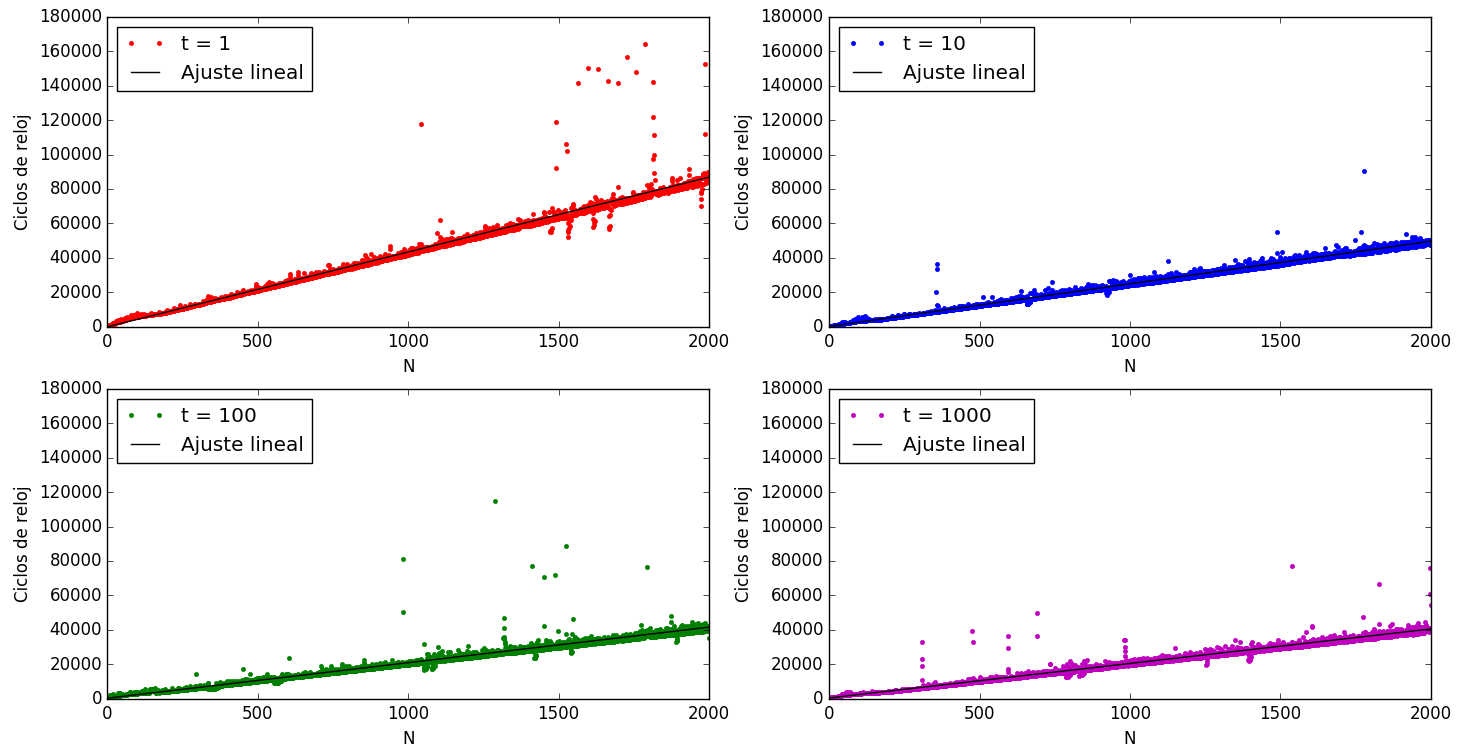
\includegraphics[width=\textwidth]{p2_2_1}
\caption{Gráfico obtenido a partir de las mediciones realizadas diferentes valores de $t$ en el problema 2}
\end{figure}

\begin{figure}[h!]
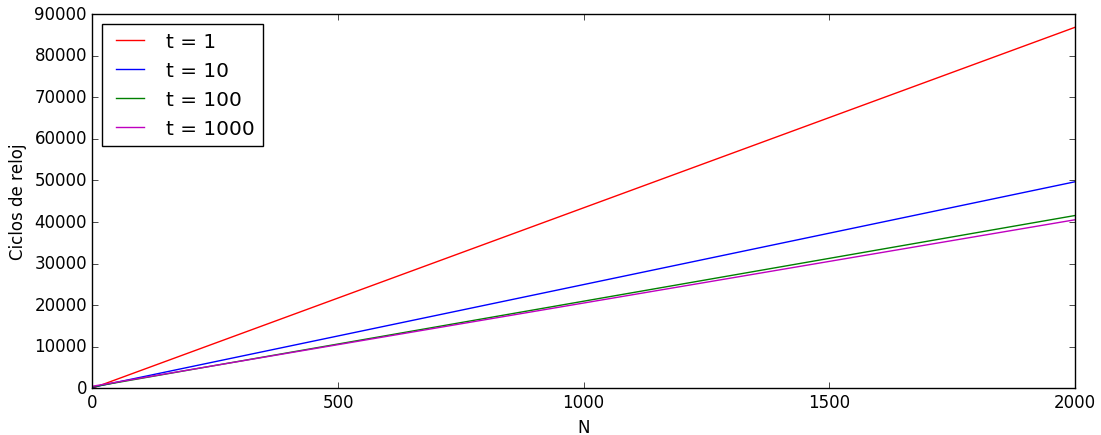
\includegraphics[width=\textwidth]{p2_2_2}
\caption{Comparación entre los ajustes lineales para los diferentes valores de $t$}
\end{figure}

Se observa que cuanto mayor es el valor de $t$, menor es la cantidad de ciclos de reloj necesarias. Esto es así ya que cada una de las genkidamas tiene un rango mayor, lo que resulta en más enemigos muertos por genkidama en promedio. Además se puede observar que el caso con $t$ = 1 está cerca del peor caso (casi 1 $N$ genkidamas) mientras que el caso con $t$ = 1000 está cerca del mejor caso (casi 1 genkidama en total).

\begin{multicols}{2}
Comparando los valores de pendientes ajustadas y el segundo gráfico se puede ver que la pendiente decrece rápidamente al principio, llegando a alcanzar la mitad de su valor. Esto es consistente con la diferencia en complejidad entre el mejor y el peor caso, que es $O(N)$ y $O(2N)$ respectivamente.

\begin{description}
\item[Pendiente para t = 1] $\approx43,416$
\item[Pendiente para t = 10] $\approx24,727$
\item[Pendiente para t = 100] $\approx20,608$
\item[Pendiente para t = 1000] $\approx20,026$
\end{description}
\end{multicols}
%TODO : no es consistente porque antes decia 3N(lo cambie). no se cual poner u,u

\subsubsection{Mediciones con distribución constante y $t$ variable}

Se realizaron mediciones usando siempre la misma distribución generada aleatoriamente con $N$ = 2000 elementos. Se varió $t$ entre 1 y 2000 y se obtuvieron los siguientes resultados:

\begin{figure}[h!]
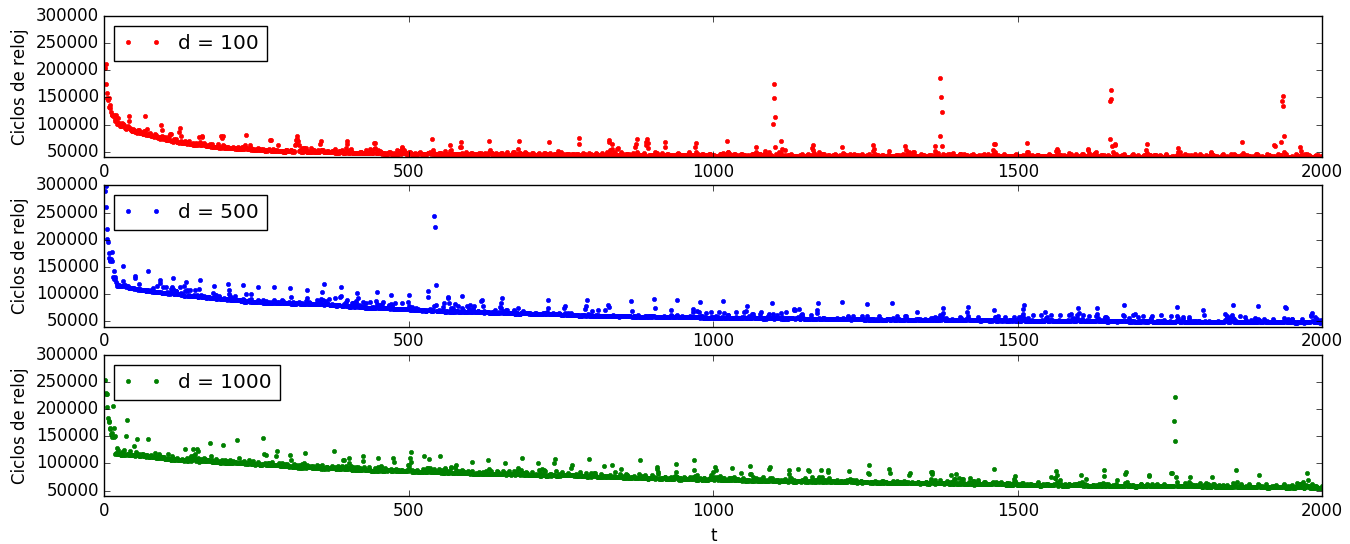
\includegraphics[width=\textwidth]{p2_3}
\caption{Mediciones para $t$ variable y distribución fija}
\end{figure}

Se observa que para $t$ cerca de 0 la cantidad de ciclos de reloj es mayor y desciende bastante cerca de $t$ = 100.% TODO no se por que pasa esto t_t 
También se ven picos periódicos. % esto no tiene sentido o33o